% !TeX root = ../main.tex

\section{Stochastic Demand Situation}
    \frame{\sectionpage}

    \begin{frame}{Method Flow}
      We aim to obtain a seat planning before the demand realization.
      \begin{itemize}
        \item The formulation of scenario-based stochastic programming(SSP).
        \item Reformulate SSP to the benders master problem(BMP) and subproblem.
        \item The optimal solution can be obtained by solving BMP iteratively.
        \item To avoid solving IP directly, we consider the linear relaxation form.
        \item Obtain integral seat planning composed of full or largest patterns by deterministic model.
      \end{itemize}
    \end{frame}

    \begin{frame}{Scenario-based Stochastic Programming}
      \footnotesize
      \begin{equation}\label{sto_form}
        \begin{aligned}
       (SSP) \max \quad & E_{\omega}\left[\sum_{i=1}^{M-1} (n_i-\delta) (\sum_{j= 1}^{N} x_{ij} + y_{i+1,\omega}^{+} - y_{i \omega}^{+}) + (n_{M}-\delta) (\sum_{j= 1}^{N} x_{Mj} - y_{M \omega}^{+})\right] \\
        \text {s.t.} \quad & \sum_{j= 1}^{N} x_{ij}-y_{i \omega}^{+}+
        y_{i+1, \omega}^{+} + y_{i \omega}^{-}=d_{i \omega}, \quad i = 1,\ldots,M-1, \omega \in \Omega \\
        & \sum_{j= 1}^{N} x_{ij} -y_{i \omega}^{+}+y_{i \omega}^{-}=d_{i \omega}, \quad i = M, \omega \in \Omega \\
        & \sum_{i=1}^{M} n_{i} x_{ij} \leq L_j, j \in \mathcal{N}\\
        & y_{i \omega}^{+}, y_{i \omega}^{-} \in \mathbb{Z}_{+}, \quad i \in \mathcal{M}, \omega \in \Omega \\
        & x_{ij} \in \mathbb{Z}_{+}, \quad i \in \mathcal{M}, j \in \mathcal{N}.
        \end{aligned}
      \end{equation}
    \end{frame}

\begin{frame}{Reformulation}
  \begin{equation}\label{BD_master}
    \begin{aligned}
  \max \quad & \mathbf{c}^{\intercal} \mathbf{x}+ z(\mathbf{x}) \\
  \text {s.t.} \quad & \mathbf{n} \mathbf{x} \leq \mathbf{L} \\
  & \mathbf{x} \in \mathbb{Z}_{+}^{M \times N},
  \end{aligned}
  \end{equation}

  where $z(\mathbf{x})$ is defined as 

$$z(\mathbf{x}) := E(z_{\omega}(\mathbf{x})) = \sum_{\omega \in \Omega} p_{\omega} z_{\omega}(\mathbf{x}),$$ and for each scenario $\omega \in \Omega$, 

  \begin{equation}\label{BD_sub}
    \begin{aligned}
      z_{\omega}(\mathbf{x}) := \max \quad & \mathbf{f}^{\intercal} \mathbf{y} \\
      \text {s.t.} \quad & \mathbf{x} \mathbf{1} + \mathbf{V} \mathbf{y} = \mathbf{d}_{\omega} \\
       & \mathbf{y} \geq 0.
    \end{aligned}
    \end{equation}
\end{frame}

\begin{frame}{Solution to Subproblem}
  Problem (3) is easy to solve with a given $\mathbf{x}$ which can be seen by the dual problem:

  \begin{equation}\label{BD_sub_dual}
    \begin{aligned}
      \min \quad & \alpha^{\intercal}_{\omega} (\mathbf{d}_{\omega}- \mathbf{x} \mathbf{1}) \\
      \text {s.t.} \quad & \alpha^{\intercal}_{\omega} \mathbf{V} \geq \mathbf{f}^{\intercal}
    \end{aligned}
    \end{equation}

    \begin{itemize}
      \item The feasible region of problem \eqref{BD_sub_dual}, $P= \{\alpha|\alpha^{\intercal} V \geq \mathbf{f}^{\intercal}\}$, is bounded. In addition, all the extreme points of $P$ are integral.
      \item The optimal solution to this problem can be obtained directly according to the complementary slackness property.
    \end{itemize}
\end{frame}

\begin{frame}{Benders Decomposition Procedure}
  \small
  Let $z_{\omega}$ be the lower bound of problem \eqref{BD_sub_dual}, SSP can be obtained by solving following restricted benders master problem:
  \begin{equation}\label{BD_master2}
    \begin{aligned}
      \max \quad & \mathbf{c}^{\intercal} \mathbf{x} + \sum_{\omega \in \Omega} p_{\omega} z_{\omega} \\
      \text {s.t.} \quad & \mathbf{n} \mathbf{x} \leq \mathbf{L} \\
      & (\alpha^{k})^{\intercal}(\mathbf{d}_{\omega}- \mathbf{x} \mathbf{1}) \geq z_{\omega}, \alpha^k \in \mathcal{O}, \forall \omega \\
       & \mathbf{x} \in \mathbb{Z}_{+}
    \end{aligned}
\end{equation} 

  Constraints will be generated from problem \eqref{BD_sub_dual} until an optimal solution is found.

  \begin{figure}[ht]
    \centering
    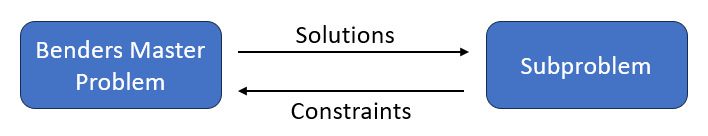
\includegraphics[width = 0.6\textwidth]{./images/BD.png}
  \end{figure}

  To avoid solving IP directly, we consider the linear relaxation of Problem \eqref{BD_master2}.
\end{frame}

% \begin{frame}{Deterministic Formulation}
%   Substitute the first constraint with $\sum_{j= 1}^{N} x_{ij} \geq s_{i}, i \in \mathcal{M}$, we can obtain the problem with lower bound supply. 
% \end{frame}

\begin{frame}{Obtain Seat Planning Composed of Full or Largest Patterns}
      \begin{description}
        \item[Step 1.] Obtain the solution, $\mathbf{x}^{*}$, by benders decomposition. Aggregate $\mathbf{x}^{*}$ to the number of each group type, ${s}_{i}^{0} =\sum_{j} x^{*}_{ij}, i \in \mathbf{M}$.

        \item[Step 2.] Solve problem \eqref{deter_upper} to obtain the optimal solution, $\mathbf{x}^{1}$. Aggregate $\mathbf{x}^{1}$ to the number of each group type, ${s}_{i}^{1} = \sum_{j} x^{1}_{ij}, i \in \mathbf{M}$.
         
        \item[Step 3.] For each row, construct a full or largest pattern.
     \end{description}
\end{frame}

\begin{frame}{Construction}
There exists an optimal solution to the stochastic programming problem such that the patterns associated with this optimal solution are composed of the full or largest patterns under any given scenarios.

Algorithm to obtain the solution of problem \eqref{full_largest}.
\end{frame}

\begin{frame}{Running time of Benders Decomposition and IP}
  \tiny
  \begin{table}[ht]
      \centering
      \begin{tabular}{|l|l|l|l|l|l|l|}
      \hline
      \# of scenarios & demands & running time of IP(s) & Benders (s) & \# of rows & \# of groups & \# of seats\\
      \hline
      1000  & (150, 350) & 5.1  & 0.13 & 30 & 8 & (21, 50)\\
      5000  & & 28.73 & 0.47 & 30 & 8 & \\
      10000 & & 66.81  & 0.91 & 30 & 8 & \\
      50000 & & 925.17 & 4.3 & 30 & 8 & \\
      \hline
      1000  & (1000, 2000) & 5.88 & 0.29 & 200 & 8 & (21, 50)\\
      5000  & & 30.0 & 0.62 & 200 & 8 & \\
      10000 & & 64.41 & 1.09 & 200 & 8 & \\
      50000 & & 365.57 & 4.56 & 200 & 8 & \\
      \hline
      1000  & (150, 250) & 17.15  & 0.18 & 30 & 16 & (41, 60) \\
      5000  & & 105.2  & 0.67 & 30 & 16 & \\
      10000 & & 260.88 & 1.28 & 30 & 16 & \\
      50000 & & 3873.16 & 6.18 & 30 & 16 & \\
      \hline
      \end{tabular}
    \end{table}
\end{frame}


\begin{frame}{Verify the performance}
  To evaluate the effectiveness of the initial seat planning, we employ a dynamic situation where decisions are made based on real-time feedback. In this context, we utilize a fixed seat planning as the foundation, and then make informed decisions accordingly.
  \vspace{0.5cm}
  
  For any given seat planning, we can make the decision (by using group-type control).
  \vspace{0.5cm}
  
  Customers have more freedom to choose their seats with fixed seat planning.
\end{frame}

\begin{frame}{Feasible Seat Planning versus IP Solution}
  \scriptsize
  \begin{table}[ht]
      \begin{tabular}{|l|l|l|l|l|l|}
      \hline
      \# samples & T & probabilities & \# rows & people served by FSP & IP \\
      \hline
      1000  & 45  & [0.4,0.4,0.1,0.1] & 8 & 85.30 & 85.3 \\
      1000  & 50  & [0.4,0.4,0.1,0.1] & 8 & 97.32 & 97.32 \\
      1000  & 55  & [0.4,0.4,0.1,0.1] & 8 & 102.40 & 102.40  \\ % slow
      1000  & 60  & [0.4,0.4,0.1,0.1] & 8 & 106.70 & NA  \\
      1000  & 65  & [0.4,0.4,0.1,0.1] & 8 & 108.84 & 108.84 \\
      \hline
      1000  & 35  & [0.25,0.25,0.25,0.25] & 8 & 87.16 & 87.08 \\
      1000  & 40  & [0.25,0.25,0.25,0.25] & 8 & 101.32 & 101.24 \\
      1000  & 45  & [0.25,0.25,0.25,0.25] & 8 & 110.62 & 110.52 \\
      1000  & 50  & [0.25,0.25,0.25,0.25] & 8 & 115.46 & NA \\
      1000  & 55  & [0.25,0.25,0.25,0.25] & 8 & 117.06 & 117.26 \\
      \hline
      5000  & 300  & [0.25,0.25,0.25,0.25] & 30 & 749.76 & 749.76 \\
      5000  & 350  & [0.25,0.25,0.25,0.25] & 30 & 866.02 & 866.42 \\
      5000  & 400  & [0.25,0.25,0.25,0.25] & 30 & 889.02 & 889.44 \\
      5000  & 450  & [0.25,0.25,0.25,0.25] & 30 & 916.16 & 916.66 \\
      \hline
      \end{tabular}
  \end{table}

Each entry of people served is the average of 50 instances.
IP will spend more than 2 hours in some instances, as `NA' showed in the table.
\end{frame}

\begin{frame}{Find the optimal solution}
  We aim to find the optimal integral solution from the optimal fractional solution.
  Suppose the aggregated supply is $(X_1, \ldots, X_M)$, let $f(\bm{X}; \Omega)$ indicate the value with the scenario set, $\Omega$.
  \begin{equation*}
    \begin{aligned}
    \max \quad & f(\bm{X{'}}; \Omega) \\
    \text {s.t.} \quad & X_i -\delta \leq X_i{'} \leq X_i + \delta, i = 1,\ldots, M \\
    & \text{for all feasible} ~\bm{X{'}}
    \end{aligned}
  \end{equation*}

Use another formulation when the length of every row is the same?

$$
\begin{array}{ll}
\max & c^{\prime} \mathbf{x}+f^{\prime} \mathbf{y} \\
\text { s.t. } & \mathbf{T} \mathbf{x}+\mathbf{V}_\omega \mathbf{y}_\omega=\mathbf{D}_\omega, \omega \in \Omega \\
& \mathbf{1} \mathbf{x}=N \\
& \mathbf{x}, \mathbf{y} \geq \mathbf{0}
\end{array}
$$

\end{frame}



\begin{frame}{Example}
  
\end{frame}